\documentclass[12pt]{article}

\usepackage{graphicx}
\usepackage{listings}
\usepackage{hyperref}
\usepackage{float}
\usepackage{enumitem}

\graphicspath{ {./images/} }

\oddsidemargin 0mm
\evensidemargin 0mm
\textwidth 160mm
\textheight 200mm

\pagestyle {plain}
\pagenumbering{arabic}

\newcounter{stepnum}

\title{CS/SE 2XC3 Lab 8 Report}
\author{
  Glotov, Oleg\\ L03, 400174037\\
  \texttt{glotovo@mcmaster.ca}
  \and
  Willson, Emma\\ L02, 400309856\\
  \texttt{willsone@mcmaster.ca}
  }
\date{\today}

\begin{document}

\maketitle

This report includes the main observations that we found in this week's lab, along with the analysis of our results.

\newpage 
\section{Prim's Algorithm}
In this section, we discuss Prim's algorithm for finding the minimum spanning tree. 
\subsection{Prim's Algorithm Version 1}
**Explanation of how algorithm works and its time complexity**
\subsection{List vs. Min Heap}
The most expensive functions in the implementation of Prim's algorithm are finding and updating the weight of the minimum edge. Our first implementation uses a list of edges that are sorted by weight. The algorithm re-sorts this list for every edge visited. Our second implementation uses a heap of nodes that are sorted by edge weight. The algorithm calls \verb+build_heap()+ at the beginning of its visitation to each node. The Python \verb+sort()+ function has a similar time complexity to \verb+build_heap()+, $O(nlogn)$.
\begin{figure}[H]
\centering
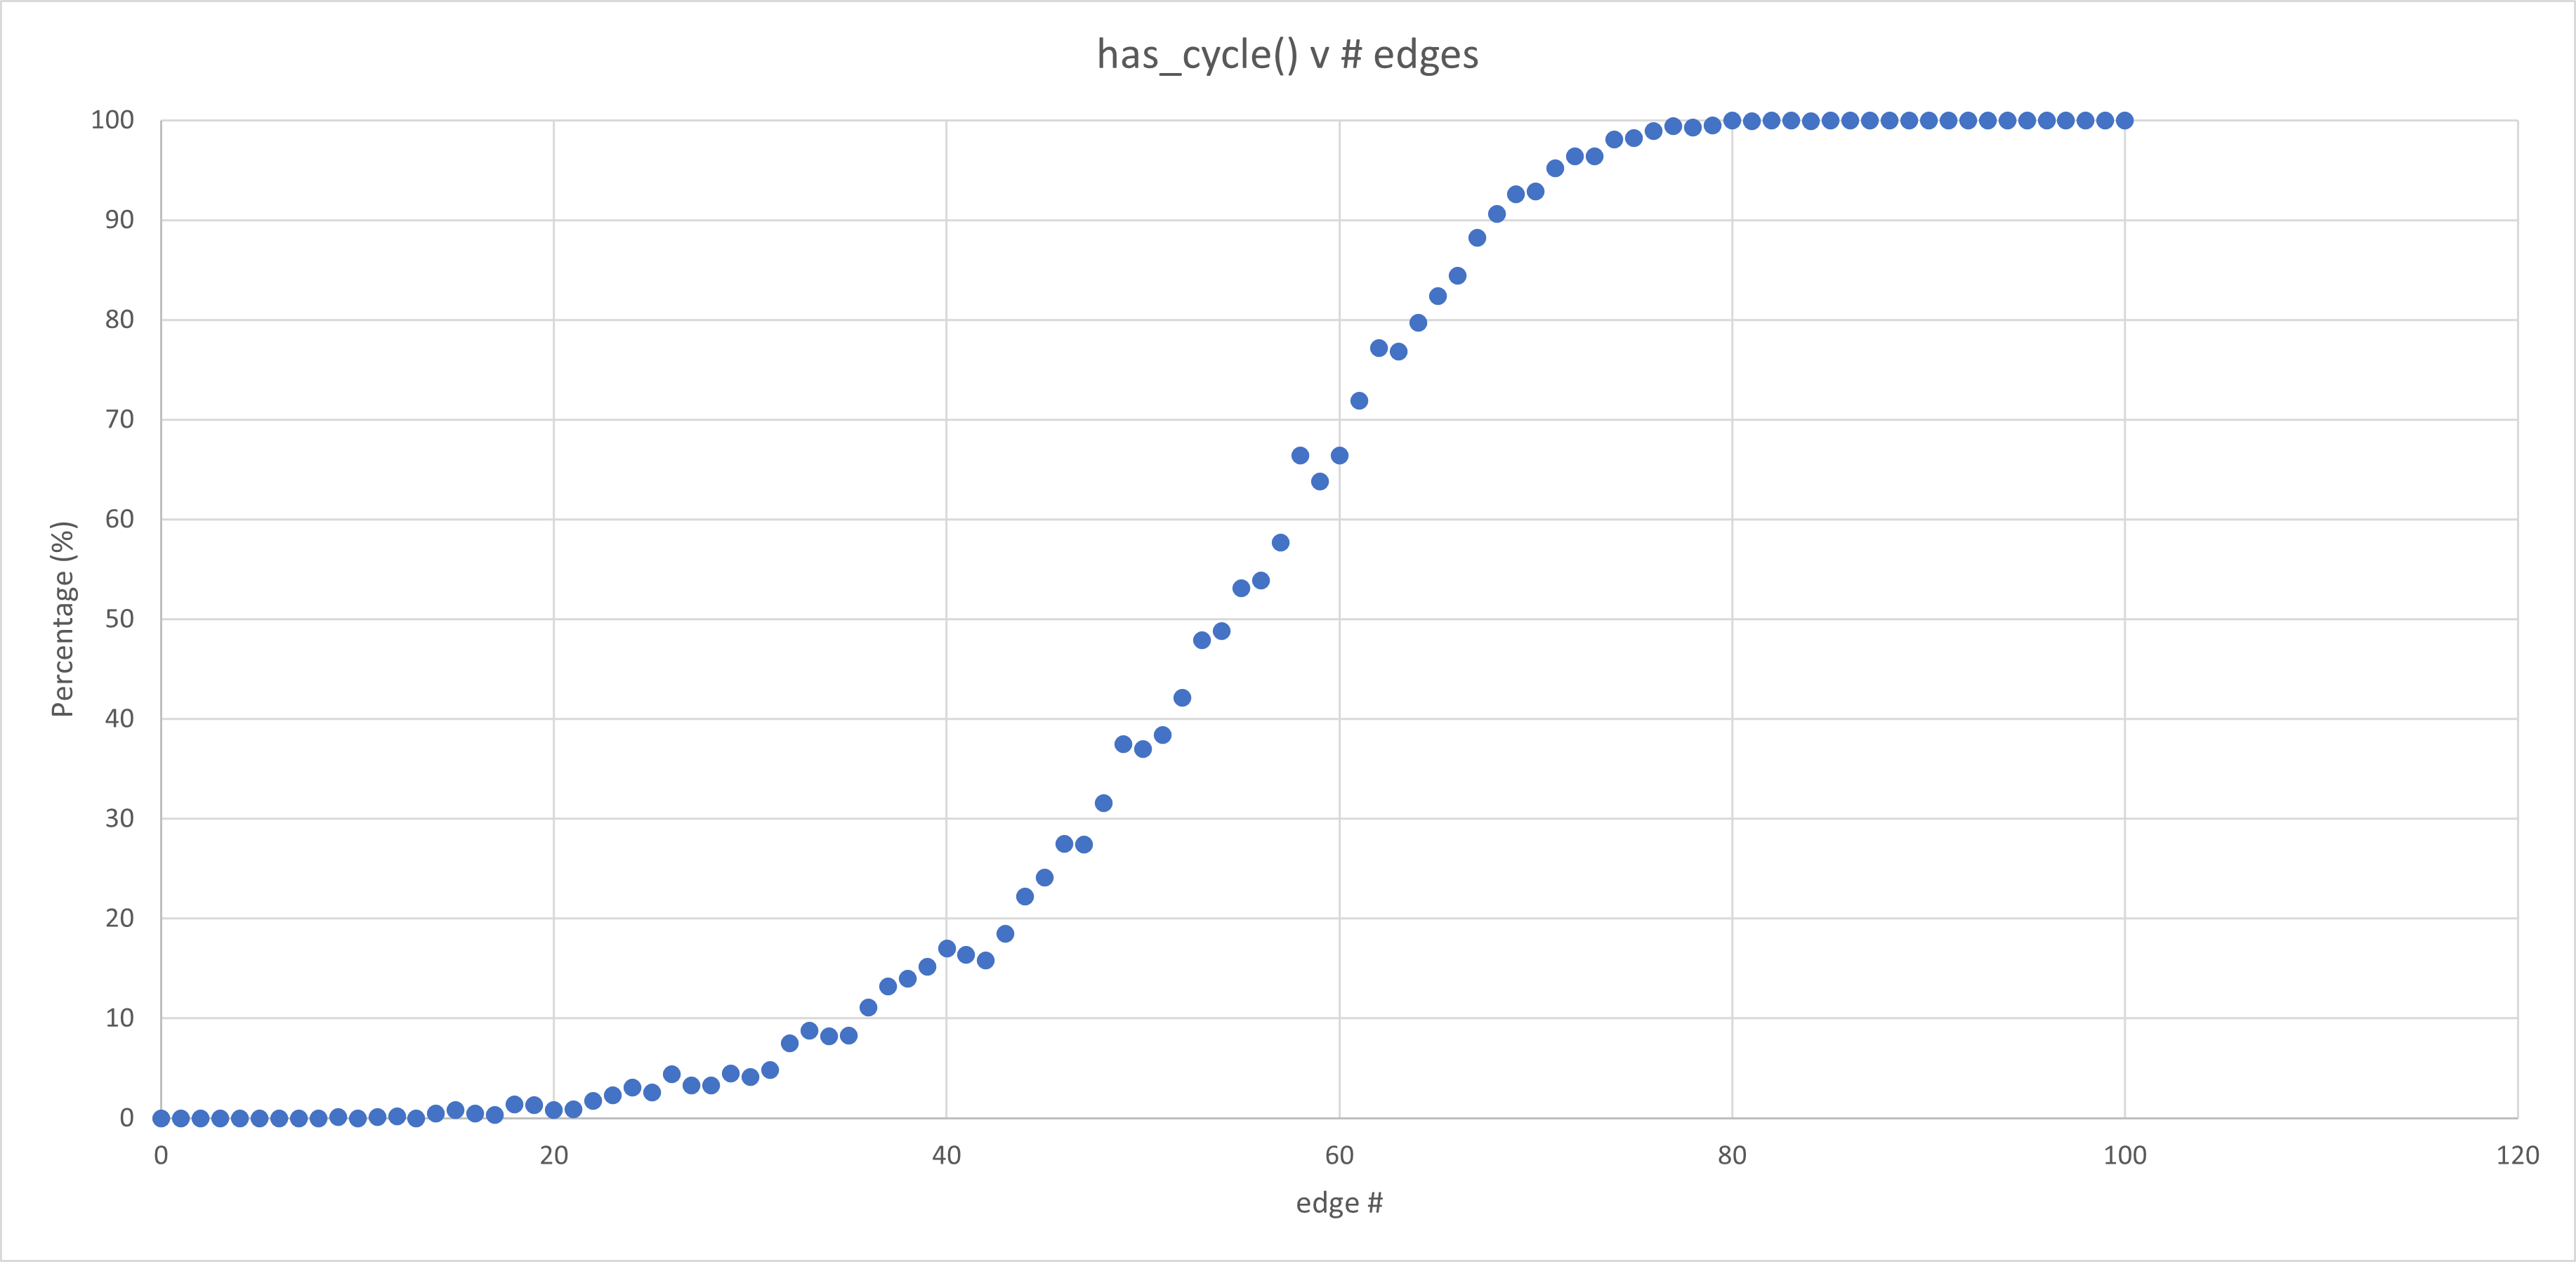
\includegraphics[width=0.9\textwidth,height=\textheight,keepaspectratio]{cycle}
\caption{time complexity of prim v1 vs. prim v2}
\label{Figure: m1}
\end{figure}
\noindent As shown in the graph above, ... 

\end{document}

